\documentclass[hyperref=colorlinks]{beamer}
\mode<presentation>
\usetheme{iclpt}
\setbeamertemplate{navigation symbols}{}
\setbeamertemplate{headline}{
\begin{beamercolorbox}[leftskip=.2cm,rightskip=.2cm,topskip=.2cm,ht=1.1cm,dp=0.1cm,wd=\textwidth]{institute in head/foot}
  
\includegraphics[height=1cm]{icl.pdf}
  \hfill
  
\includegraphics[height=1cm]{../Pics/CMS-Color.pdf}
\end{beamercolorbox}
}
\setbeamertemplate{footline}{
\begin{beamercolorbox}[ht=.55cm,dp=0.4cm,wd=\textwidth,leftskip=.3cm]{author in head/foot}%
  \begin{minipage}[c]{5cm}%
    \usebeamerfont{author in head/foot}
    \insertshortauthor 
    \insertshorttitle
    \end{minipage}\hfill%
  \insertframenumber{} / \pageref{lastframe}
  \hfill
  \begin{minipage}{6cm}
    \hfill
  \end{minipage}
\end{beamercolorbox}%
}

\usepackage{color}
\usepackage{tabularx,colortbl}
\usepackage{graphicx}
\usepackage{pdfpages}
\usepackage{feynmp}
\DeclareGraphicsRule{*}{mps}{*}{}

\title{\vspace{-0.2cm} VBF Higgs to Invisible}
\subtitle{HIG-14-038, AN-14-243\vspace{-0.7cm}}
\author[]{}%\underline{P. Dunne}} % A.M. Magnan and A. Nikitenko Joao Pela with \\ R. Aggleton, J. Brooke: Bristol \\ C.Asawangtrakuldee, Q.Li: Peking \\ P. Srimanobhas: Chulalongkorn \\ S. Kumar, K. Mazumdar: Mumbai}
\titlegraphic{
  \vspace{-0.7cm}
  %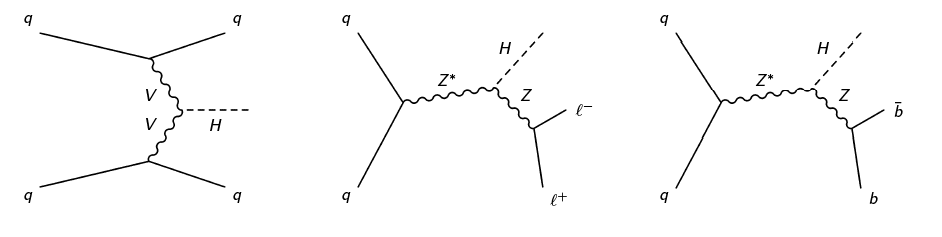
\includegraphics[width=\textwidth]{TalkPics/invcomb021213/feyndiags}
  %% \begin{fmfgraph*}(100,70)
  %%         \fmfleft{i1,i2}
  %%         \fmfright{o1,o2,o3}
  %%         \fmf{fermion}{i1,v1,o1}
  %%         \fmf{fermion}{i2,v2,o3}
  %%         \fmf{phantom,tension=4/5}{v1,v2}
  %%         \fmffreeze
  %%         \fmf{photon,label=$W,,Z$}{v1,v3}
  %%         \fmf{photon,label=$W,,Z$}{v2,v3}
  %%         \fmf{dashes}{v3,o2}
  %%         \fmflabel{$q$}{i1}
  %%         \fmflabel{$q$}{i2}
  %%         \fmflabel{$q$}{o1}
  %%         \fmflabel{$q$}{o3}
  %%         \fmflabel{$H$}{o2}
  %%       \end{fmfgraph*}
}
\date{}
\begin{document}
\begin{fmffile}{higgsexoupdatefeyndiags}

%TITLE PAGE
\section{Title}
\begin{frame}
  \titlepage
  
\end{frame}

\begin{frame}
  \frametitle{Overview}
  \begin{block}{}
    \scriptsize
    \begin{itemize}
    \item We predict almost twice as many $\mu\nu$ events than $e\nu$ events
    \item[-] $W\rightarrow\mu\nu$: $101.8 \pm 6.1 \pm 12.2$, $W\rightarrow e\nu$: $57.4 \pm 7.3 \pm 6.7$
    \item Data driven scale factors are different but compatible at just over $1 \sigma$ when systematics are accounted for
    \item We see a significant difference in the signal region MC yield (24\% difference) 
    \item It was suggested that we separate events by gen lepton in/outside acceptance
    \item[-] If difference is due to ID we should see no difference outside acceptance
    \end{itemize}
  \end{block}
  \centering
\end{frame}

\begin{frame}
  %NEVENTS INSIDE VS OUTSIDE, GOOD AGREEMENT INSIDE ACCEPTANCE, BAD OUTSIDE
  \frametitle{Inside/outside acceptance check}
  \begin{block}{}
    \scriptsize
    \begin{itemize}
    \item Check MC yield in signal region from  $W\rightarrow e/\mu\nu$
    \item[-] i.e. we veto any reconstructed leptons
    \item Split into events with gen lepton inside acceptance ($|\eta|<2.1$) and outside acceptance ($|\eta|>2.4$)
    \end{itemize}
    \begin{center}
      \begin{tabular}{|l|c|c|}
        \hline
        Process & Inside acceptance & Outside acceptance \\
        \hline
        $W\rightarrow e\nu$ & $73.7\pm 6.8$ &  {\textcolor{red}{$30.2\pm 4.9$}} \\
        \hline
        $W\rightarrow \mu\nu$ & $61.5\pm 6.8$ & $74.4\pm 7.3$ \\
        \hline
      \end{tabular}
      \end{center}
      \begin{itemize}
      \item Inside acceptance results are as expected:
      \item[-] slightly more e$\nu$ events
      \item[-] this is because electron ID efficiency is lower so fewer events are vetoed
      \item Outside acceptance results not as expected:
      \item[-] outside acceptance there are a lot fewer $e\nu$ events than $\mu\nu$
      \end{itemize}
  \end{block}
\end{frame}


\begin{frame}
  \frametitle{Distributions inside acceptance}
  \vspace{-.3cm}
  \begin{center}
    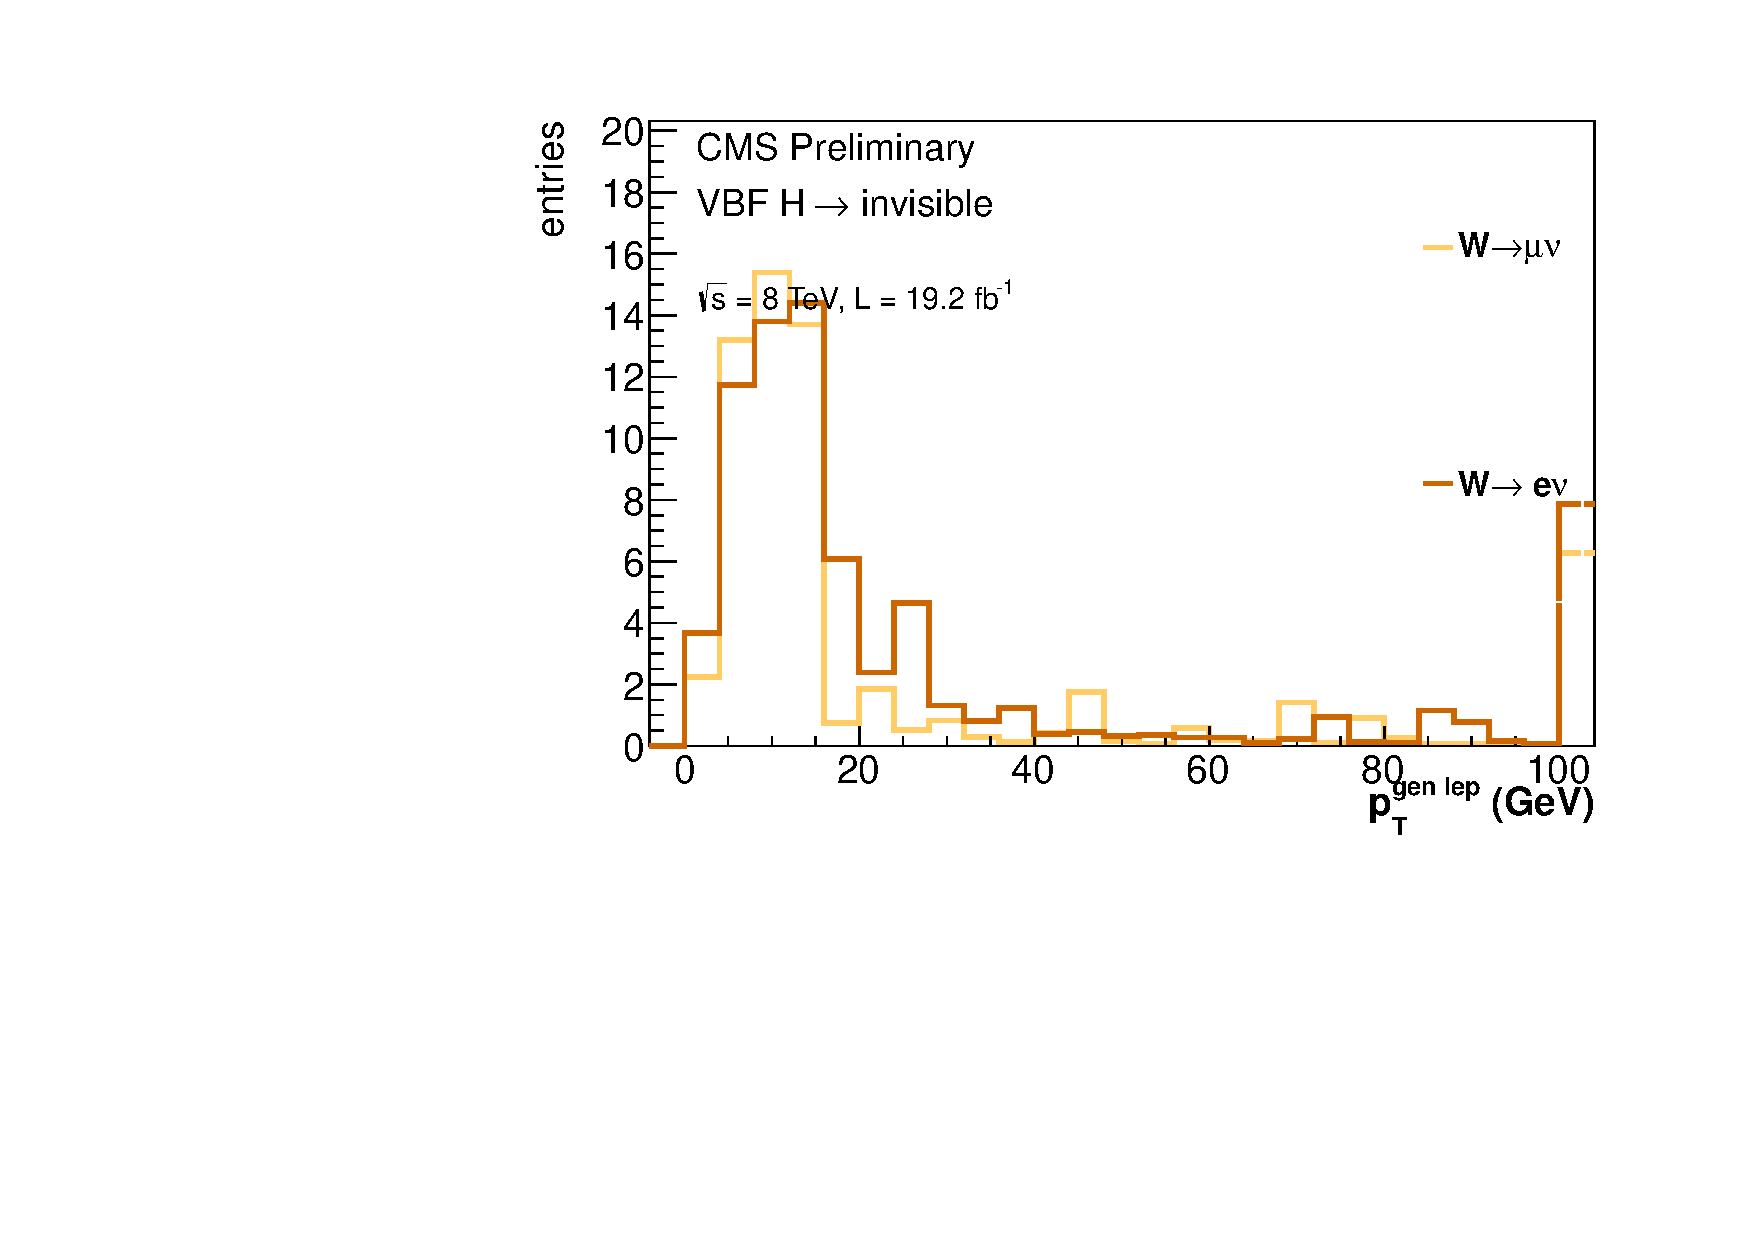
\includegraphics[width=.4\textwidth,clip=true,trim=0 0 0 30]{TalkPics/genlepstudy020315/insideacceptancetightdphi/nunu_genlep1_pt.pdf}
    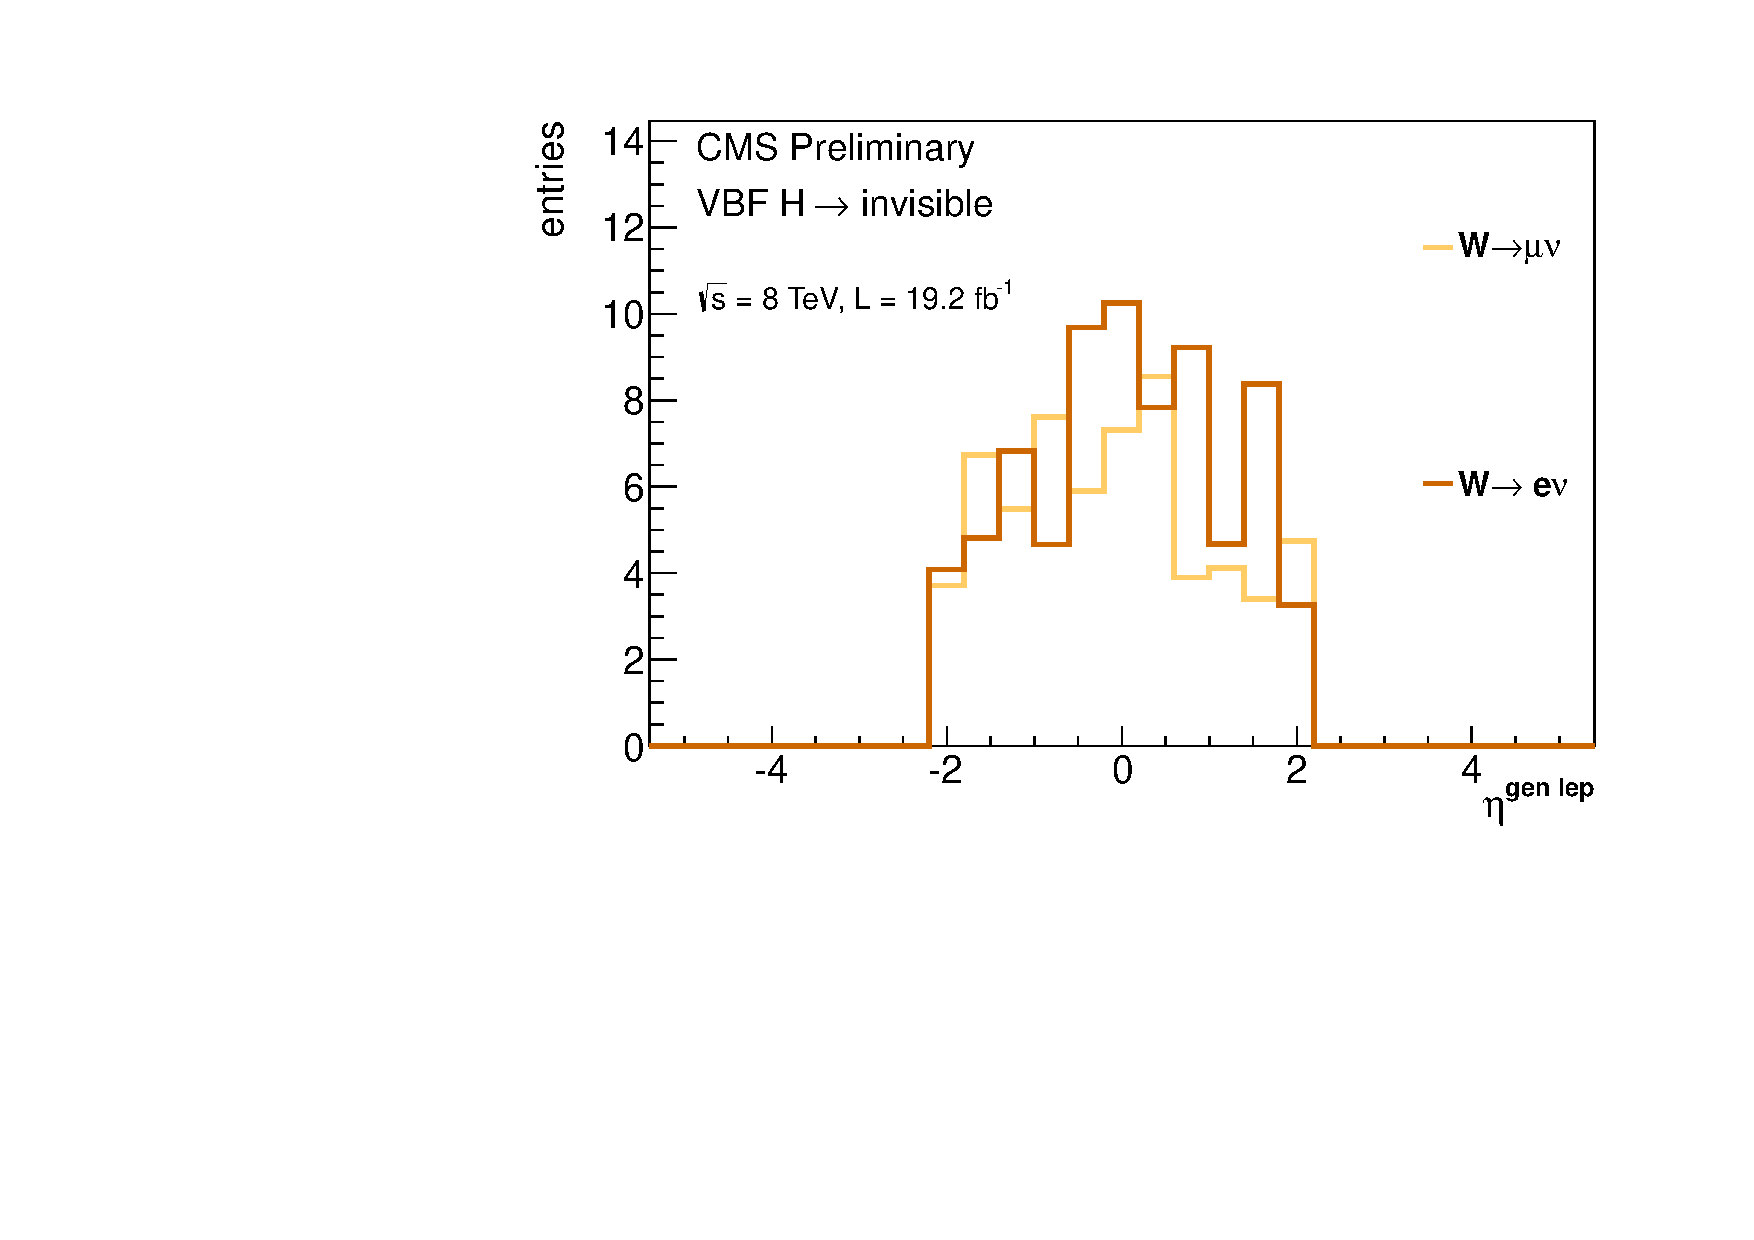
\includegraphics[width=.4\textwidth,clip=true,trim=0 0 0 30]{TalkPics/genlepstudy020315/insideacceptancetightdphi/nunu_genlep1_eta.pdf}

    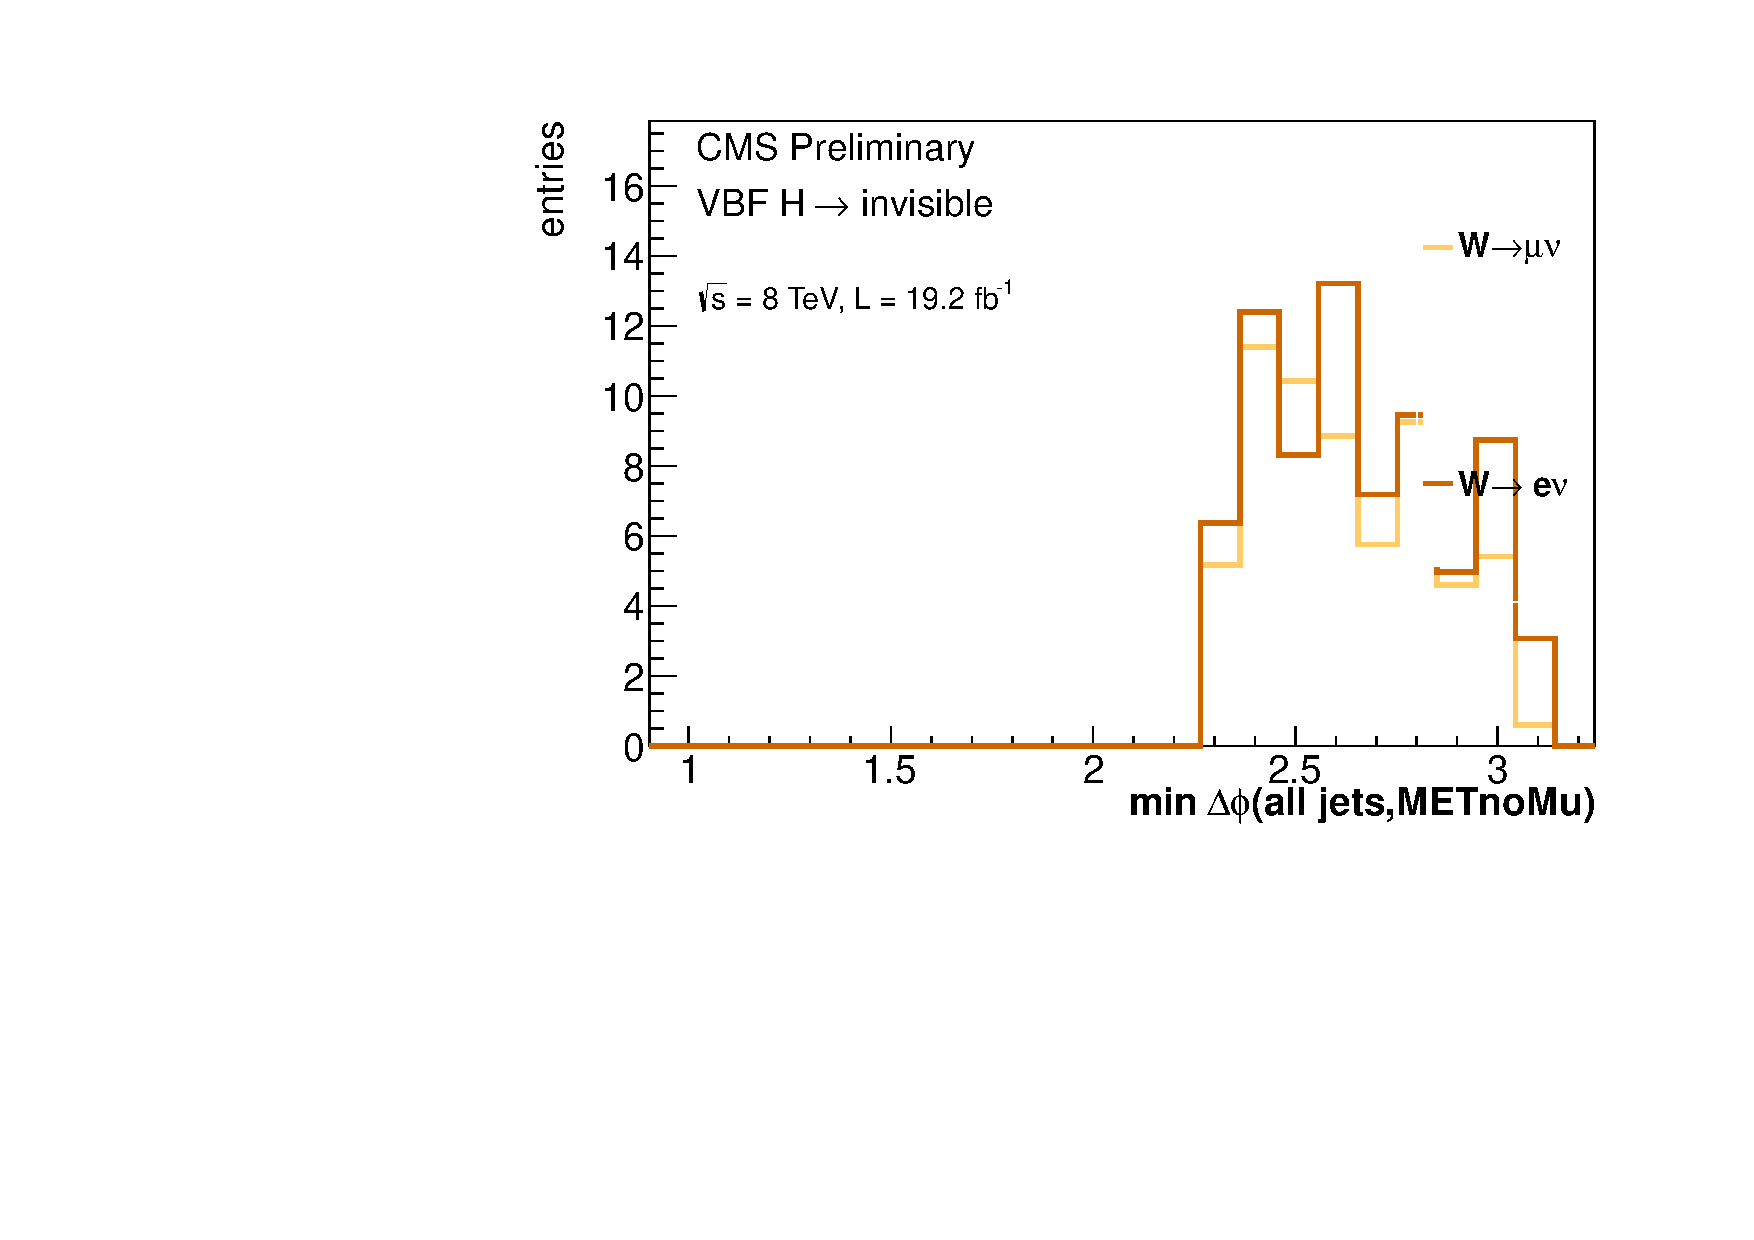
\includegraphics[width=.4\textwidth,clip=true,trim=0 0 0 30]{TalkPics/genlepstudy020315/insideacceptancetightdphi/nunu_alljetsmetnomu_mindphi.pdf}
    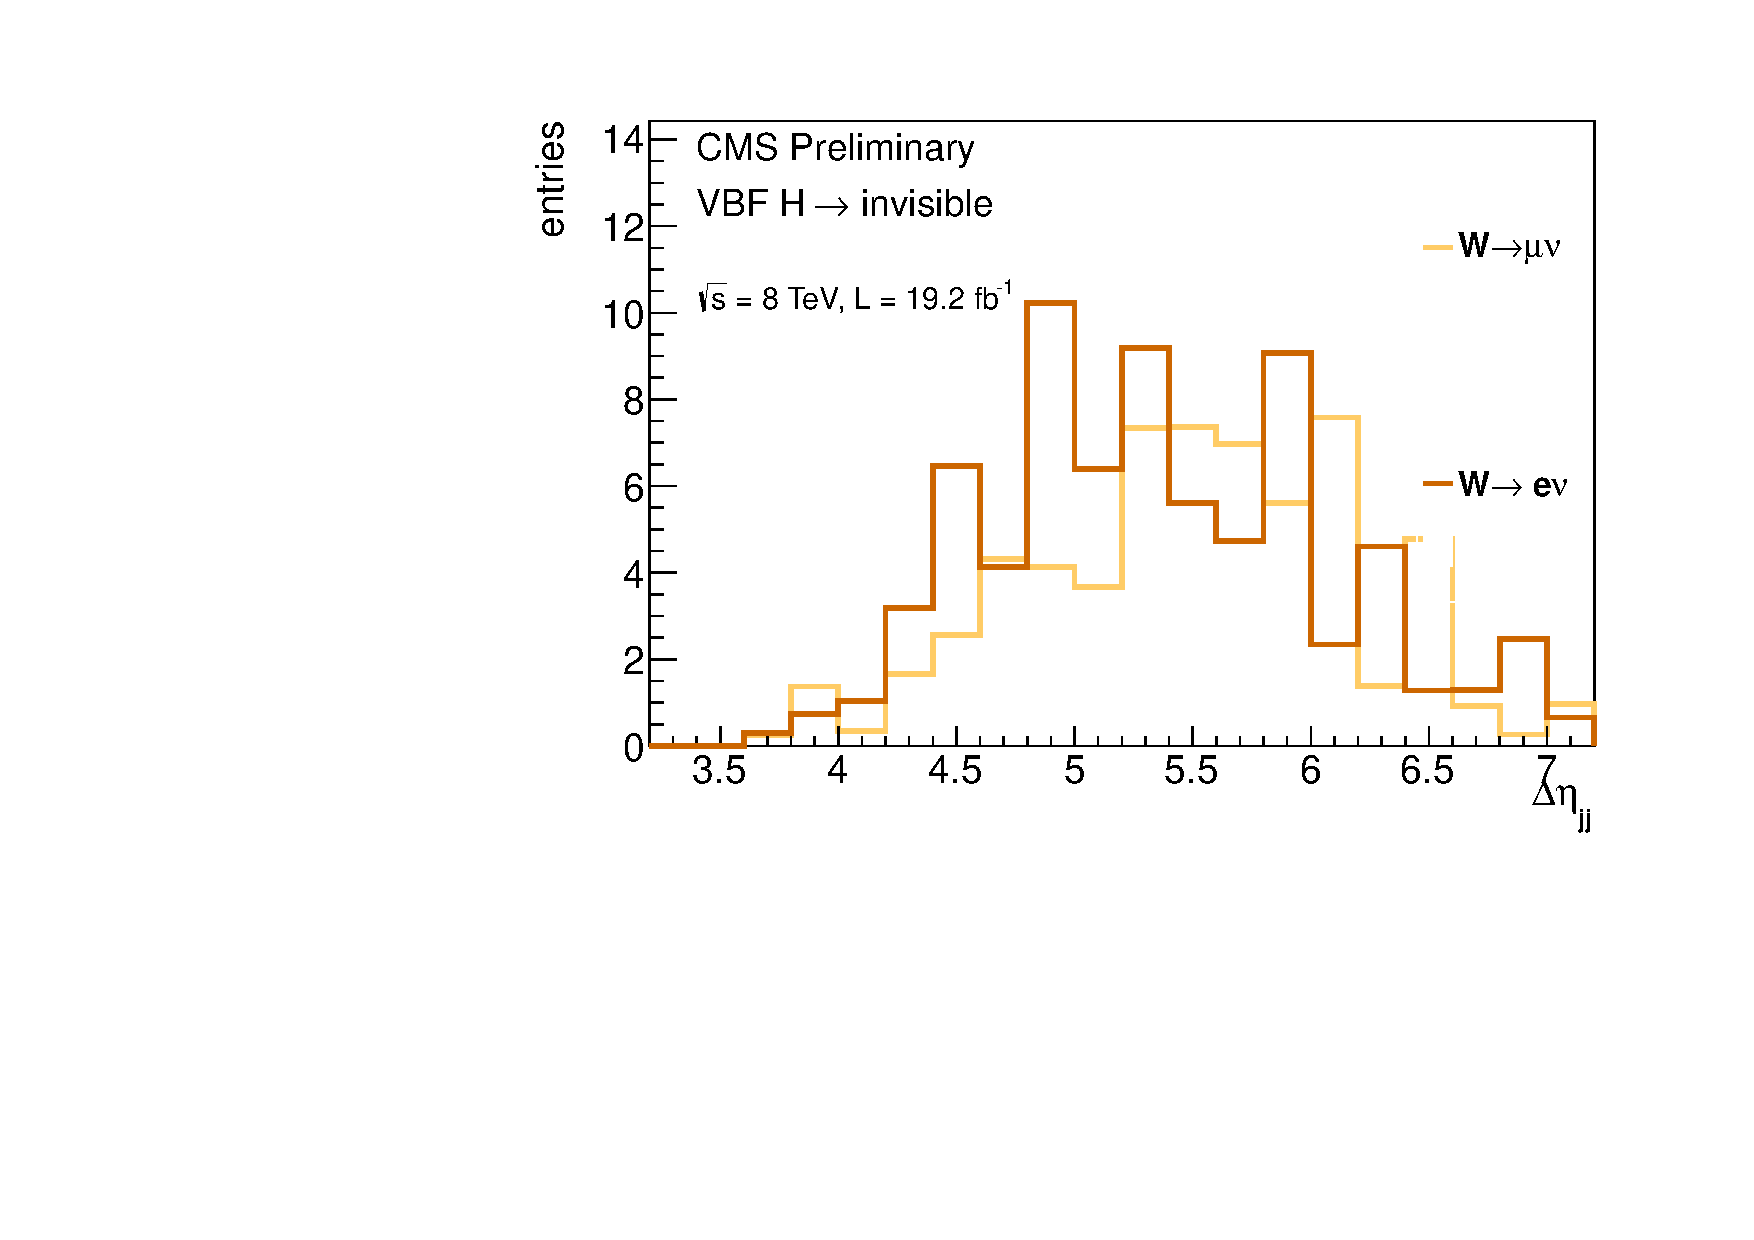
\includegraphics[width=.4\textwidth,clip=true,trim=0 0 0 30]{TalkPics/genlepstudy020315/insideacceptancetightdphi/nunu_dijet_deta.pdf}
    \end{center}
  %!!FIRST SHOW GOOD SHAPE AGREEMENT INSIDE, E MU EFF NOT SAME SO EXPECTED
  \begin{block}{}
    \scriptsize
    \begin{itemize}
    \item Shape agreement is also reasonably good inside acceptance
    \end{itemize}
  \end{block}

\end{frame}

\begin{frame}
  %!!SHOW NJETS, MINDPHI, GENLEPPT AS EVIDENCE FOR ELE BECOMING JETS OUTSIDE ACCEPTANCE
  \frametitle{Distributions outside acceptance}
  \vspace{-.7cm}
  \begin{center}
    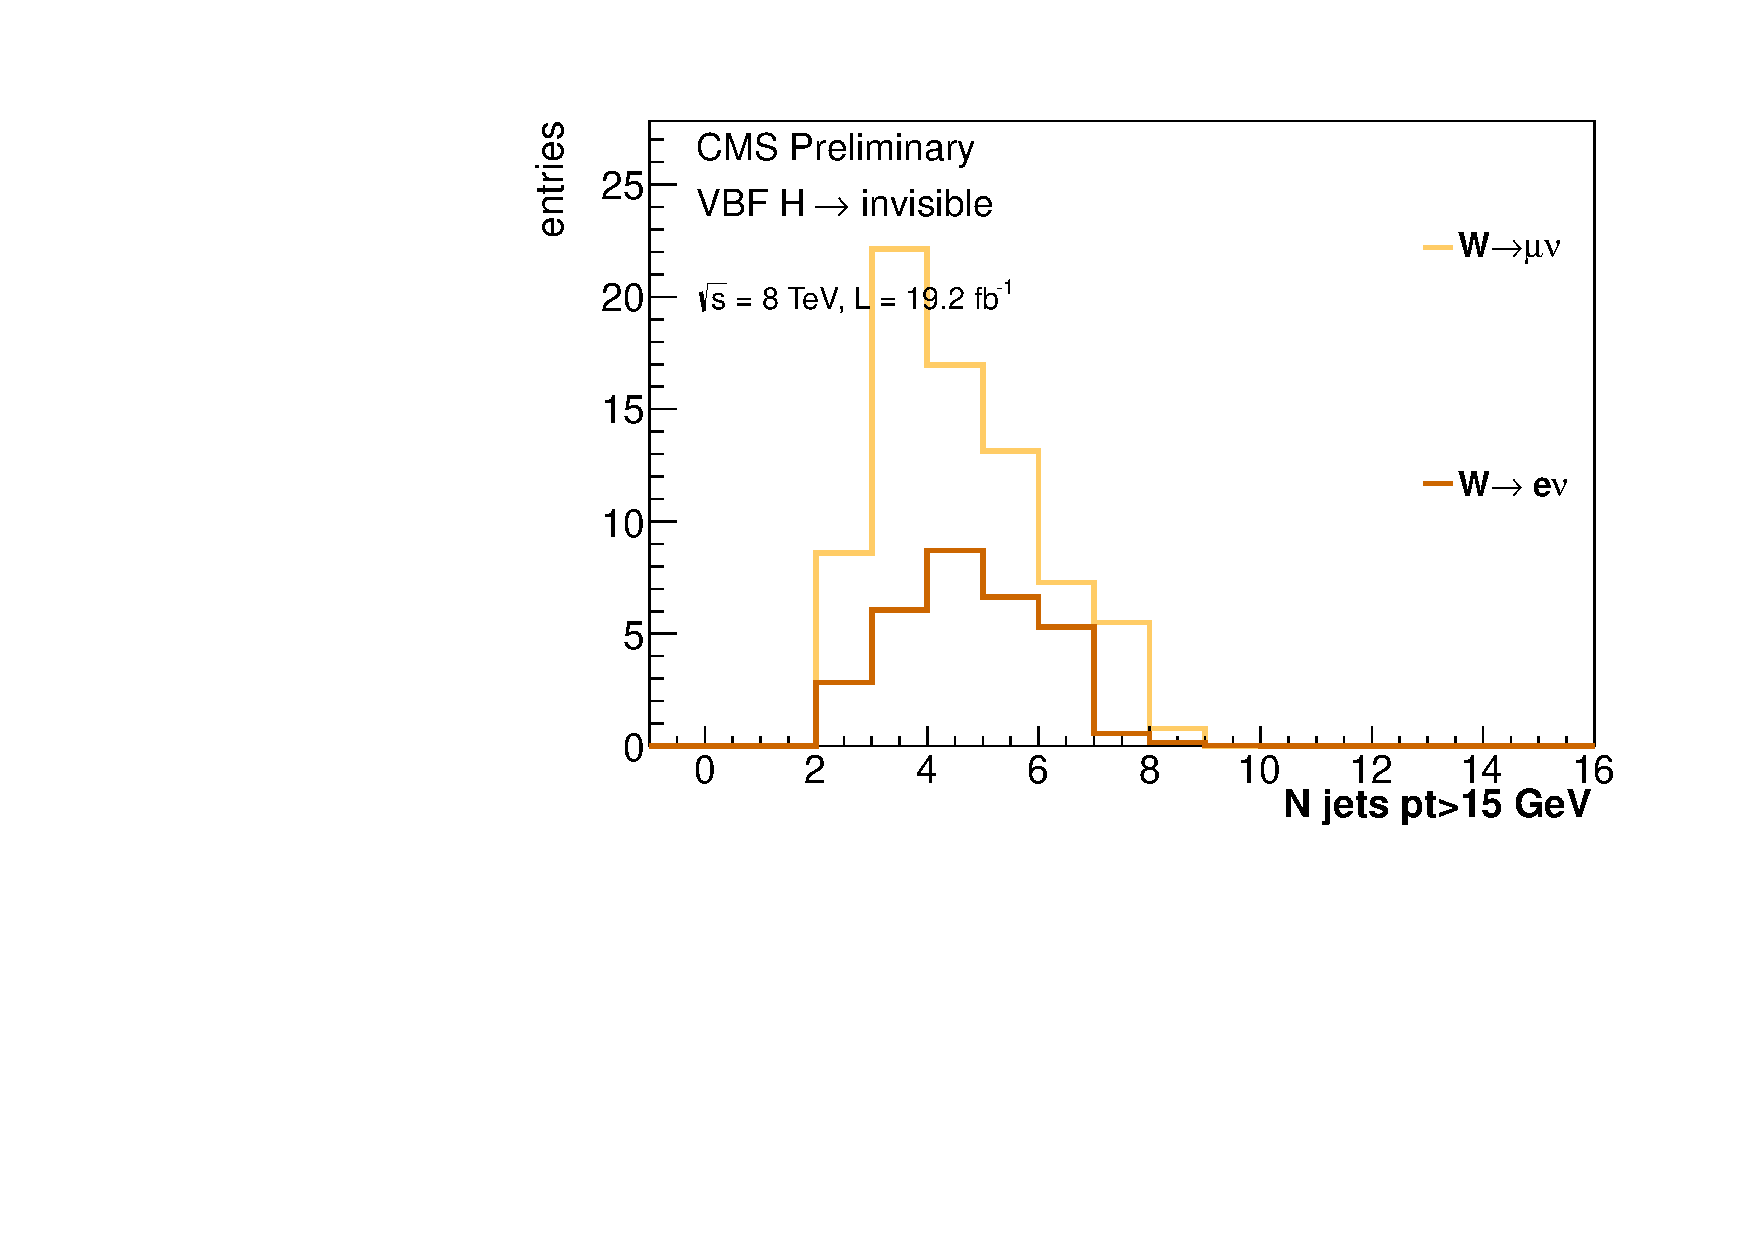
\includegraphics[width=.5\textwidth,height=.45\textheight,clip=true,trim=0 0 0 30]{TalkPics/genlepstudy020315/outsideacceptancetightdphi/nunu_n_jets_15.pdf}
    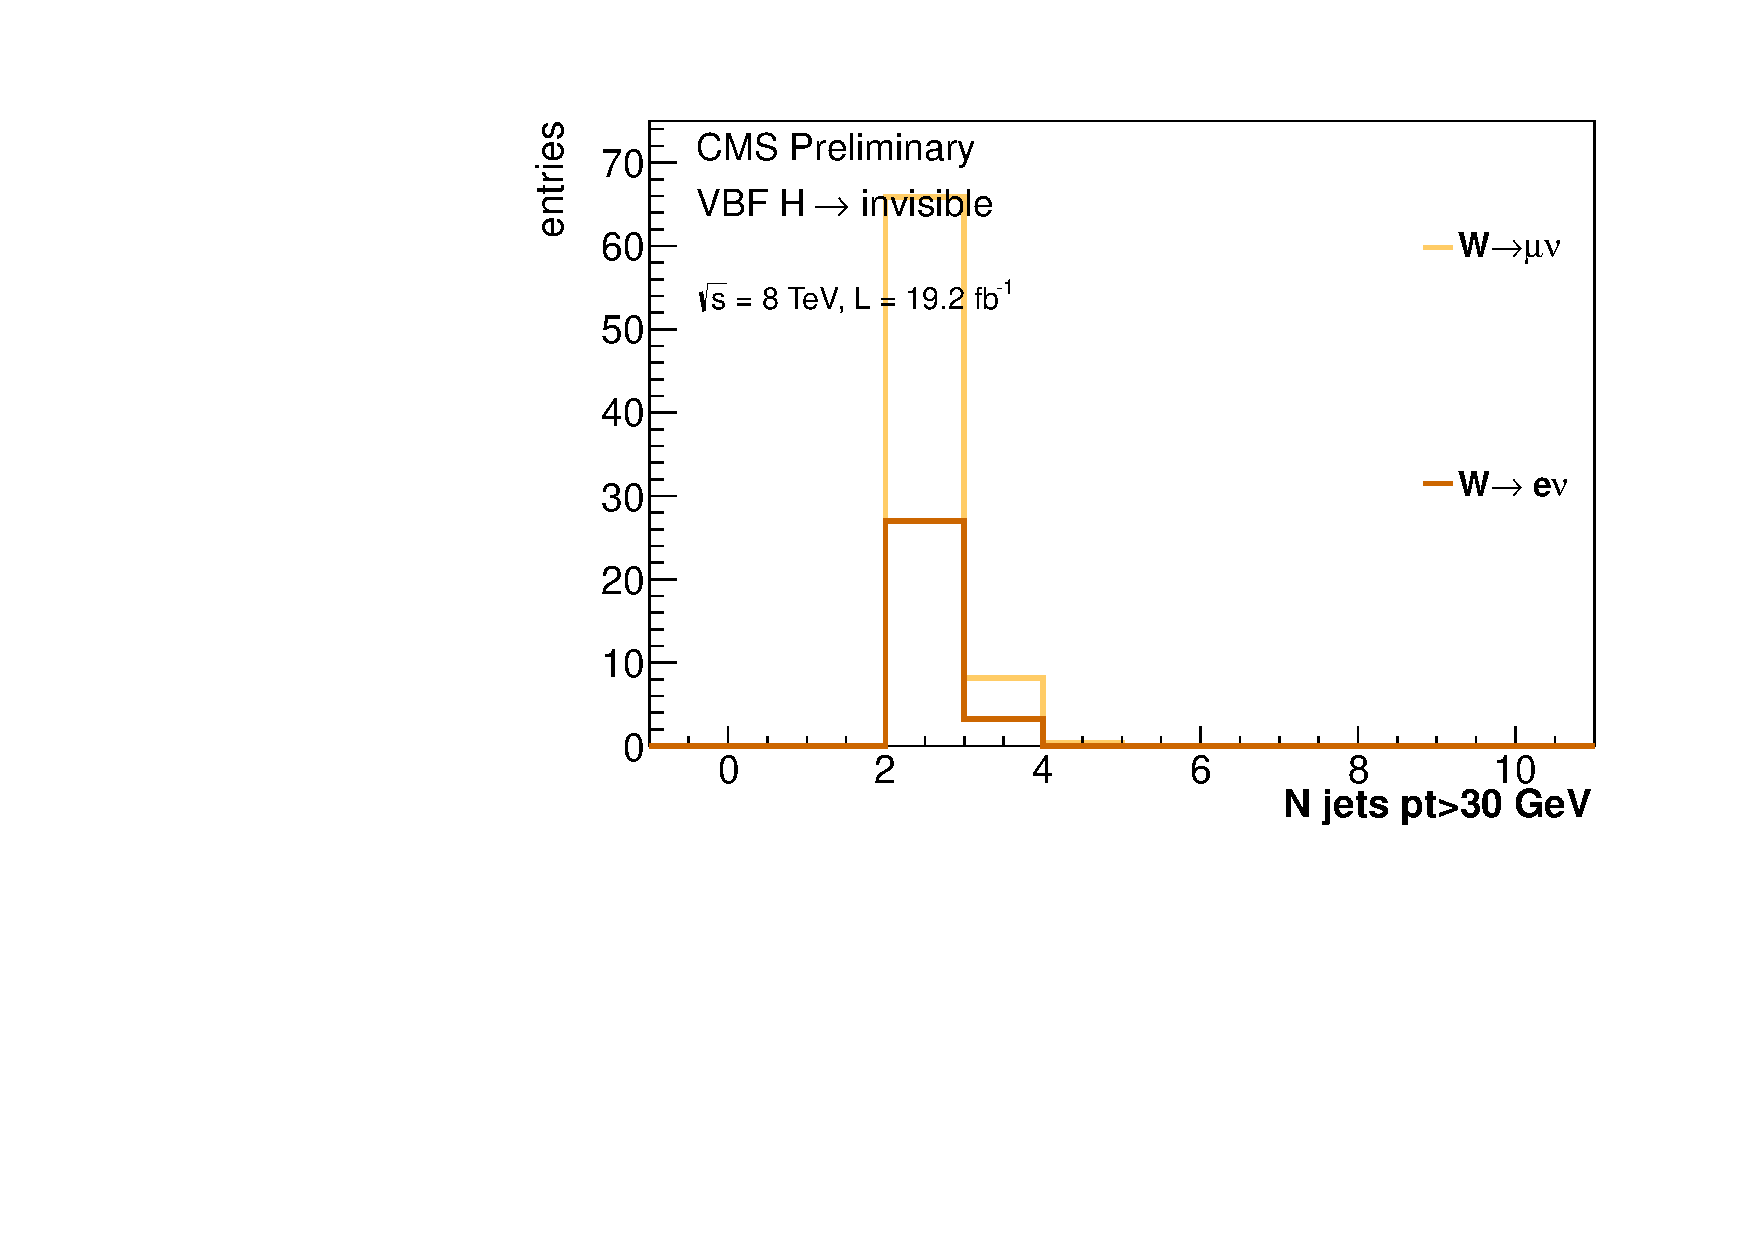
\includegraphics[width=.5\textwidth,height=.45\textheight,clip=true,trim=0 0 0 30]{TalkPics/genlepstudy020315/outsideacceptancetightdphi/nunu_n_jets_30.pdf}


    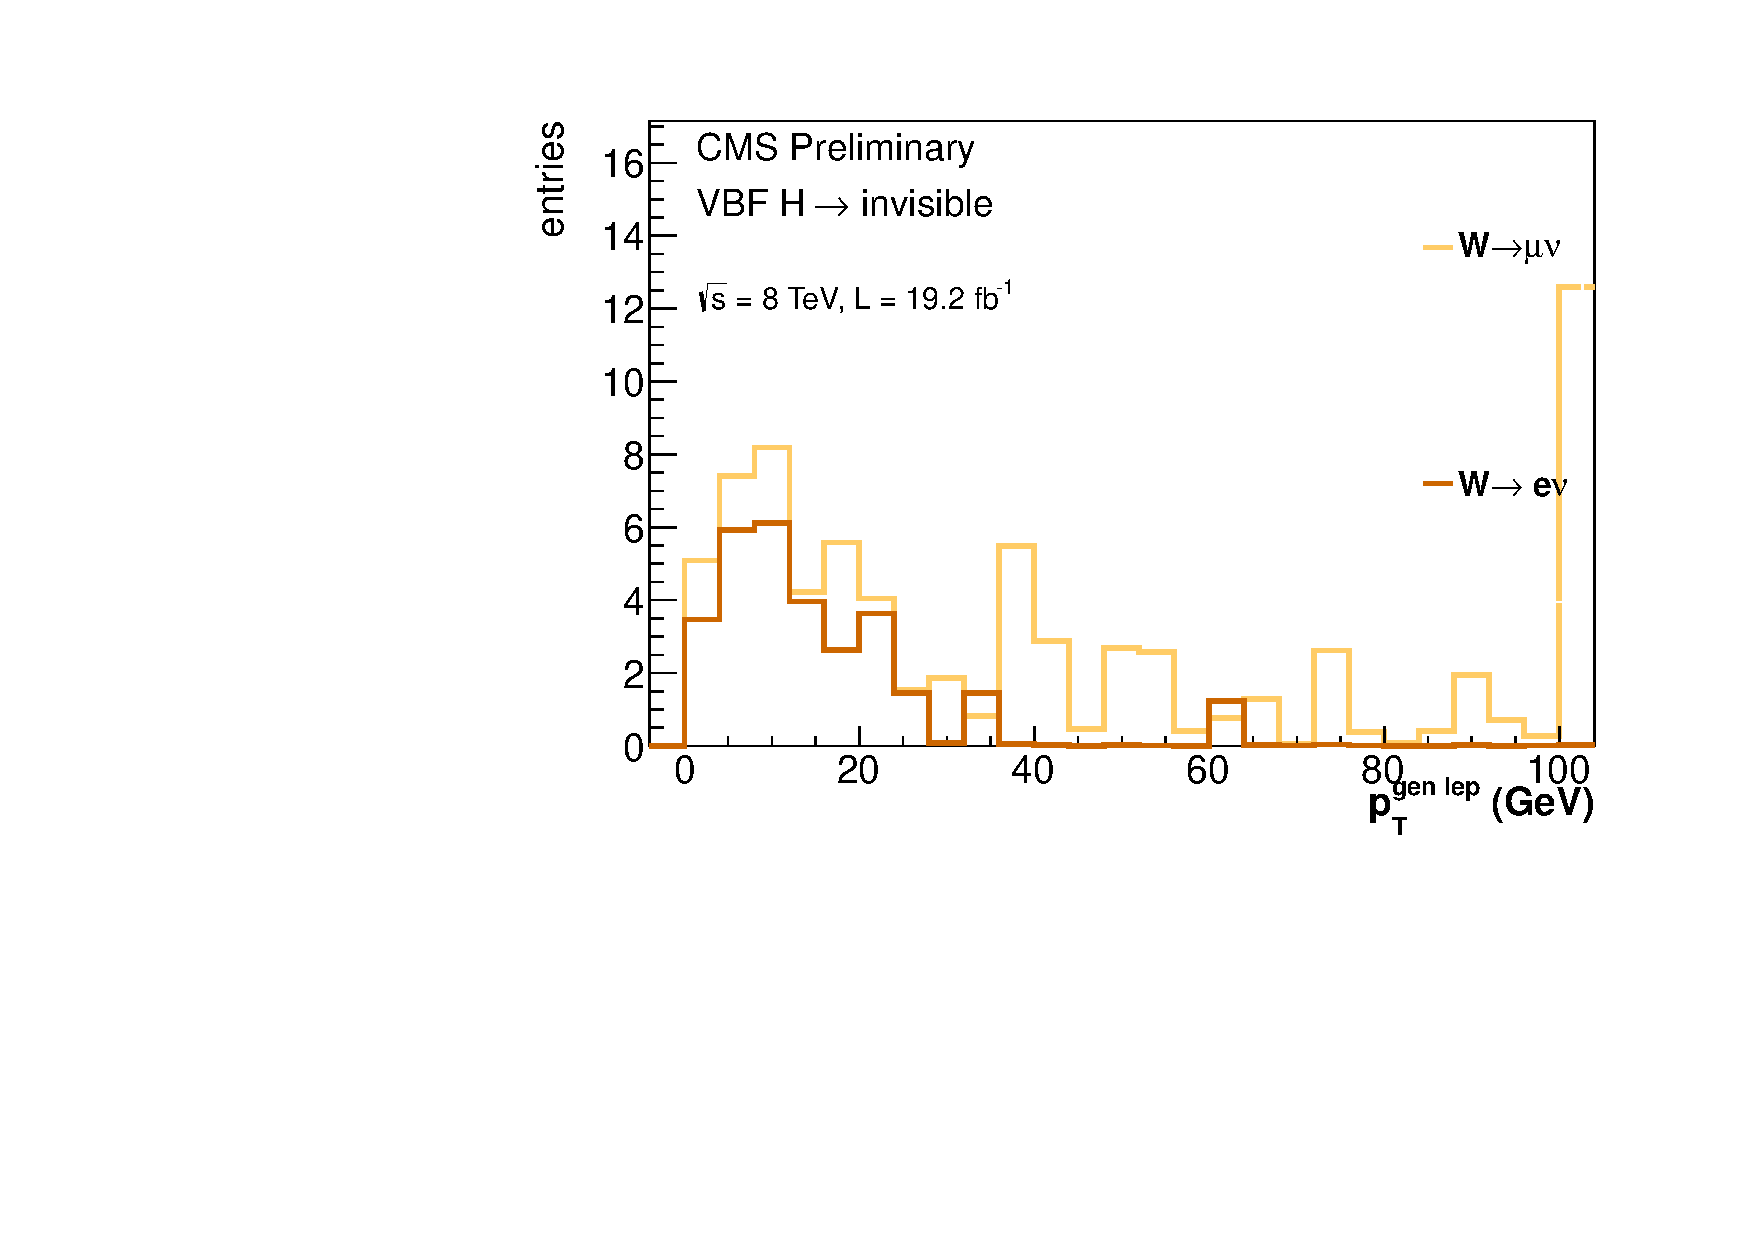
\includegraphics[width=.5\textwidth,height=.45\textheight,clip=true,trim=0 0 0 30]{TalkPics/genlepstudy020315/outsideacceptancetightdphi/nunu_genlep1_pt.pdf}
    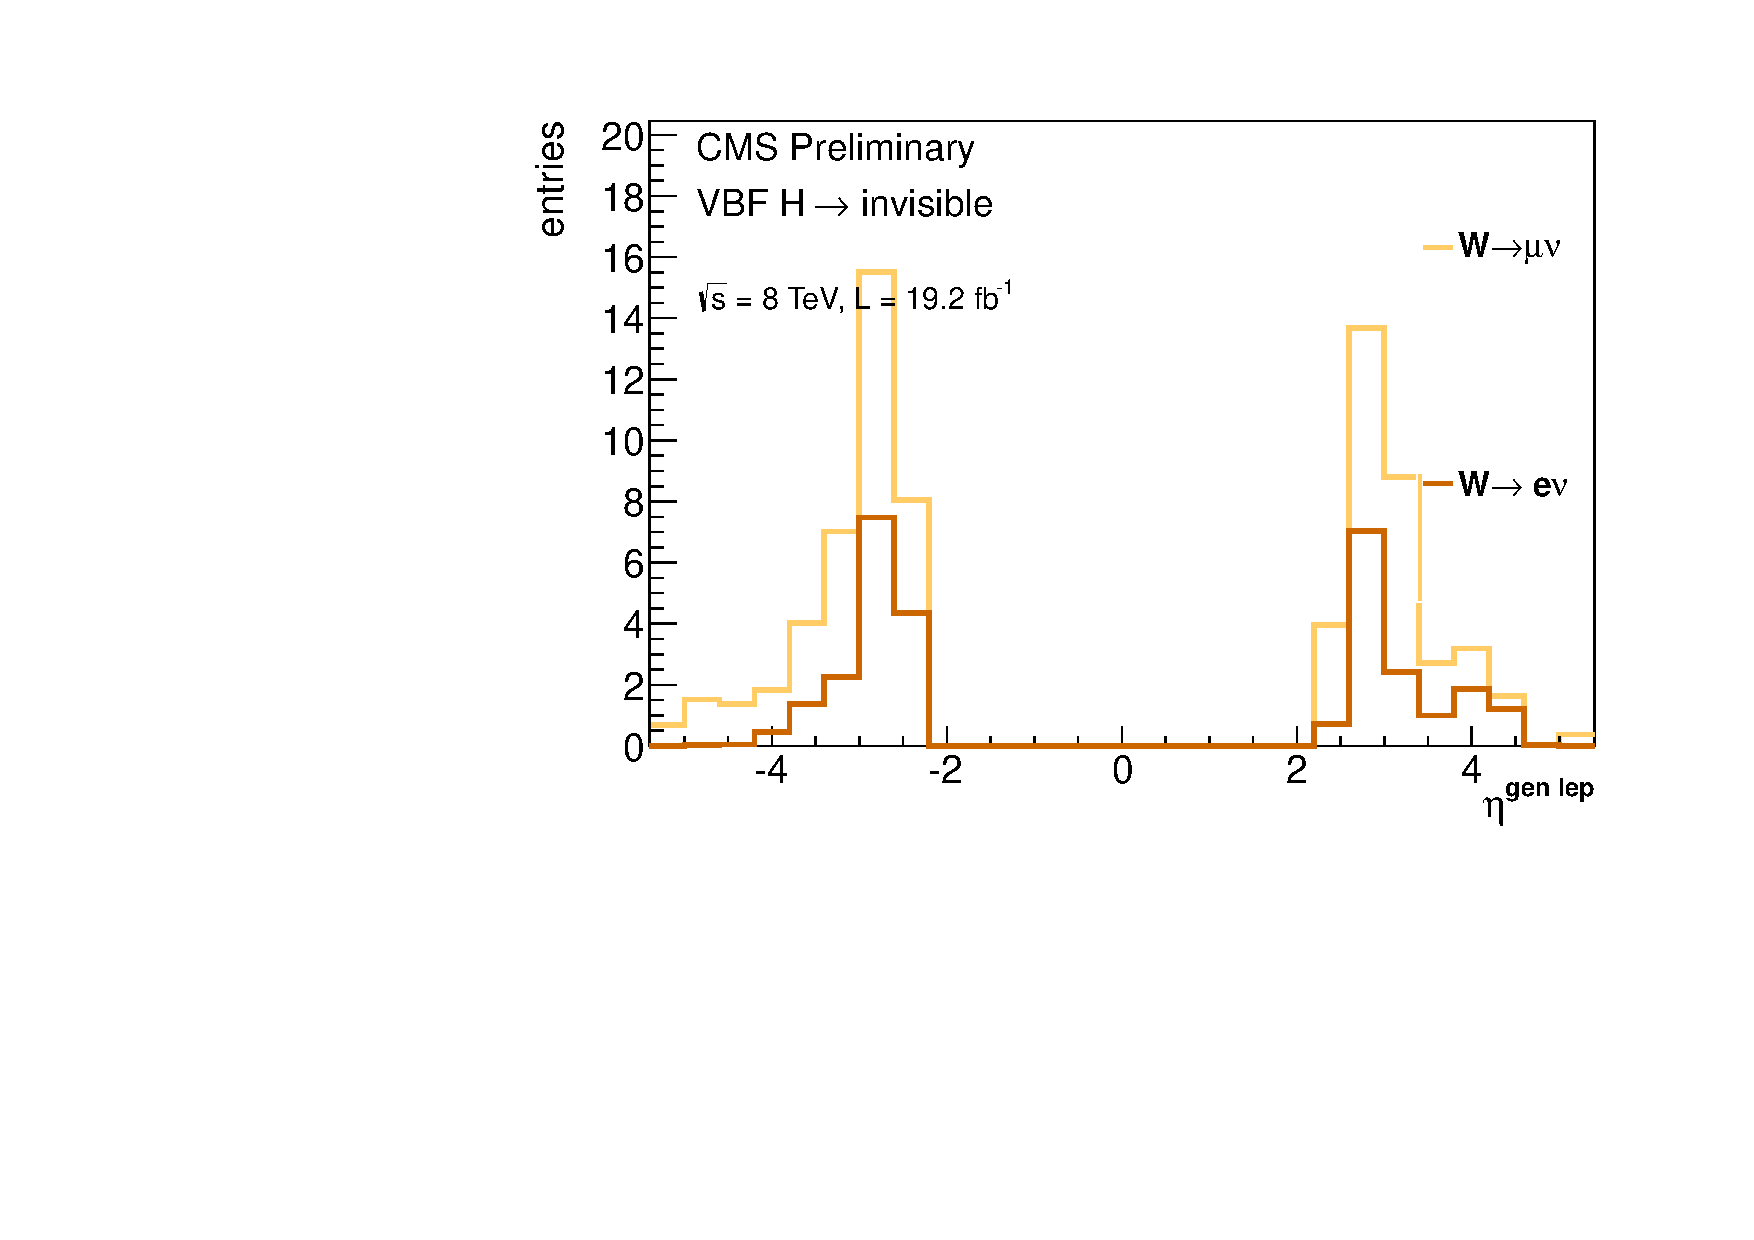
\includegraphics[width=.5\textwidth,height=.45\textheight,clip=true,trim=0 0 0 30]{TalkPics/genlepstudy020315/outsideacceptancetightdphi/nunu_genlep1_eta.pdf}
    \end{center}

\end{frame}

\begin{frame}
  \frametitle{Analysis of outside acceptance distributions}
  \begin{block}{}
    \scriptsize
    \begin{itemize}
    \item Outside acceptance $e\nu$ events have a lot more jets
    \item No $e\nu$ events with gen lepton $p_{T}$ much higher than 30 GeV
    \item We believe this is because outside acceptance electrons are often reconstructed as jets
    \item[-] this is much rarer for muons
    \item Extra jets then cause the event to fail the jetmetdphi cut
    \item As a further check jetmetdphi was loosened to check that this cut was rejecting $e\nu$ events
    \end{itemize}
  \end{block}

\end{frame}

\begin{frame}
  %!!SHOW NJETS, MINDPHI, GENLEPPT AS EVIDENCE FOR ELE BECOMING JETS OUTSIDE ACCEPTANCE
  \frametitle{Outside acceptance - jetmetphi$>1$}
    \begin{columns}
      \column{1.1\textwidth}
      \begin{center}
        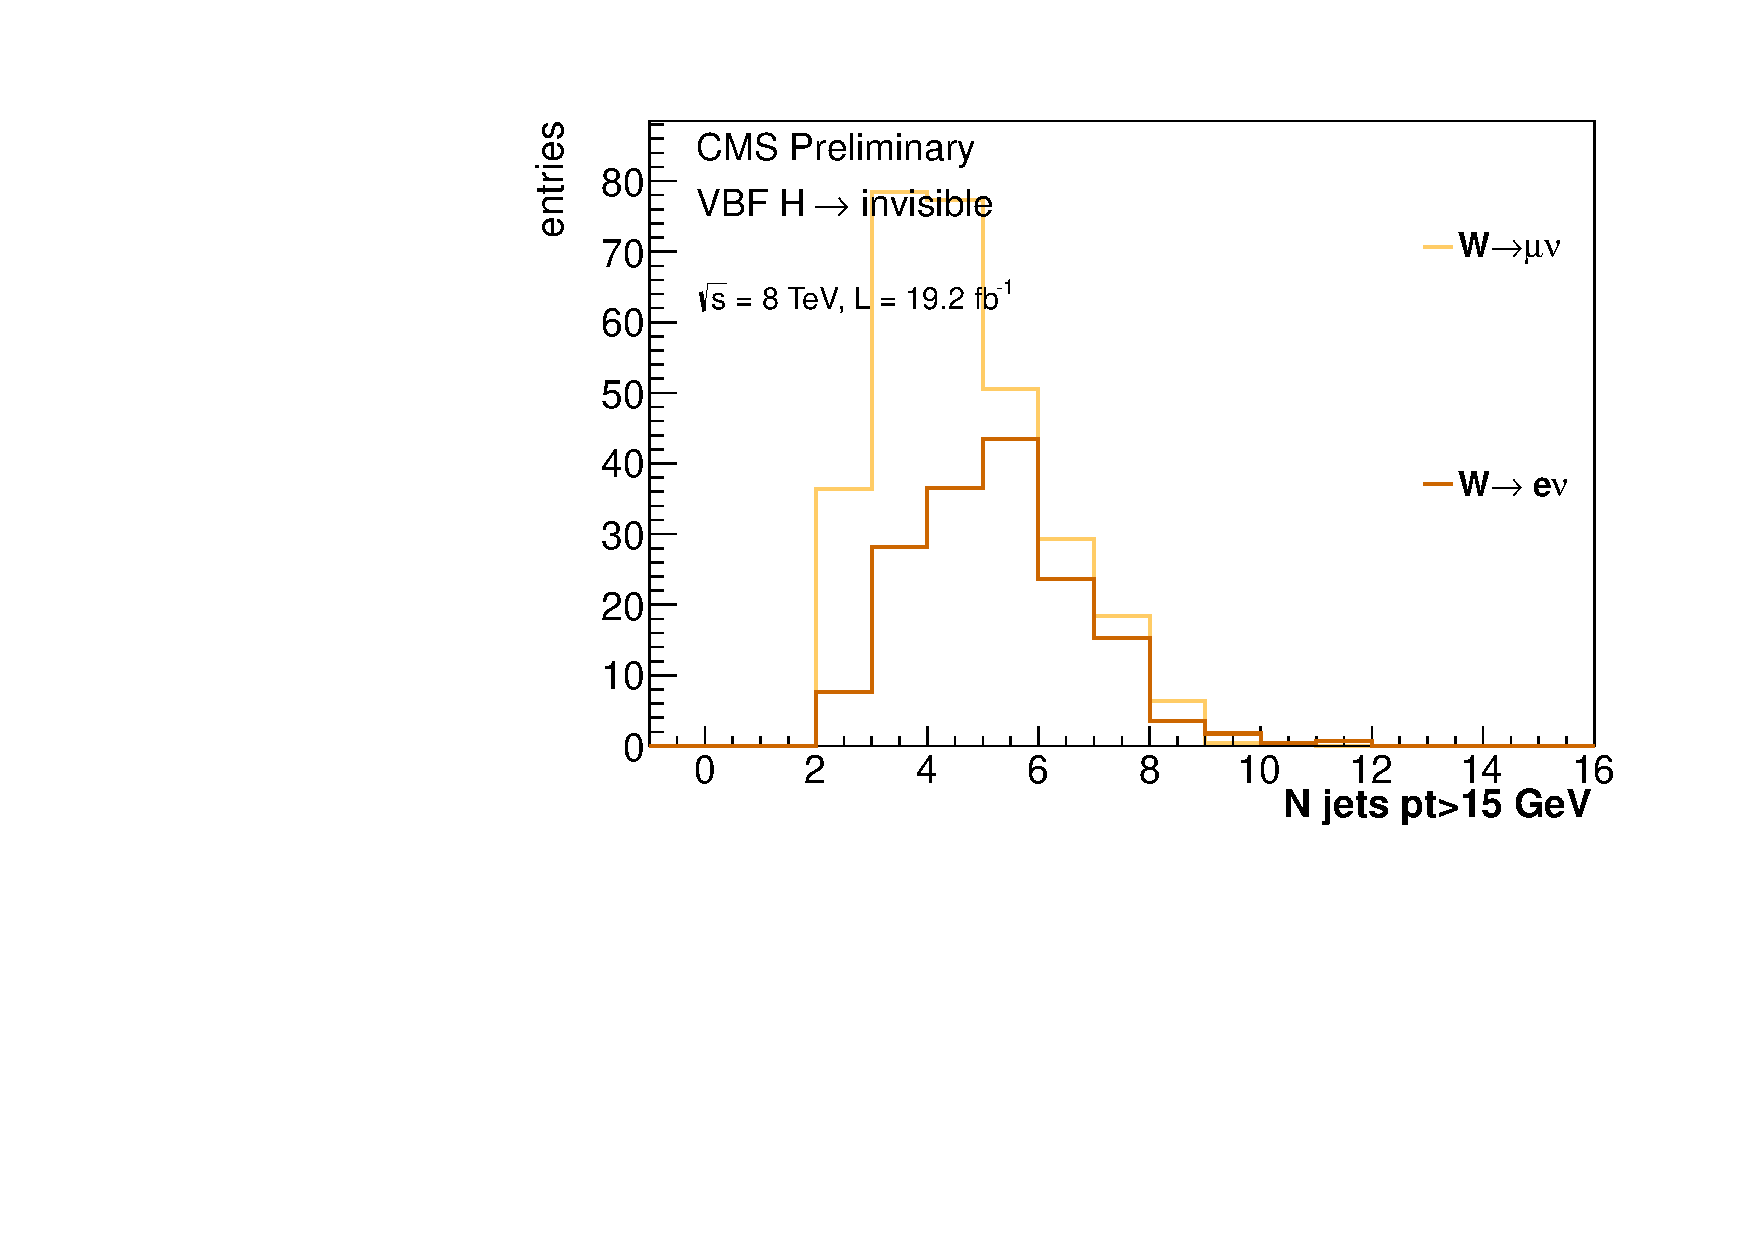
\includegraphics[width=.35\textwidth,clip=true,trim=0 0 0 30]{TalkPics/genlepstudy020315/outsideacceptance/nunu_n_jets_15.pdf}
        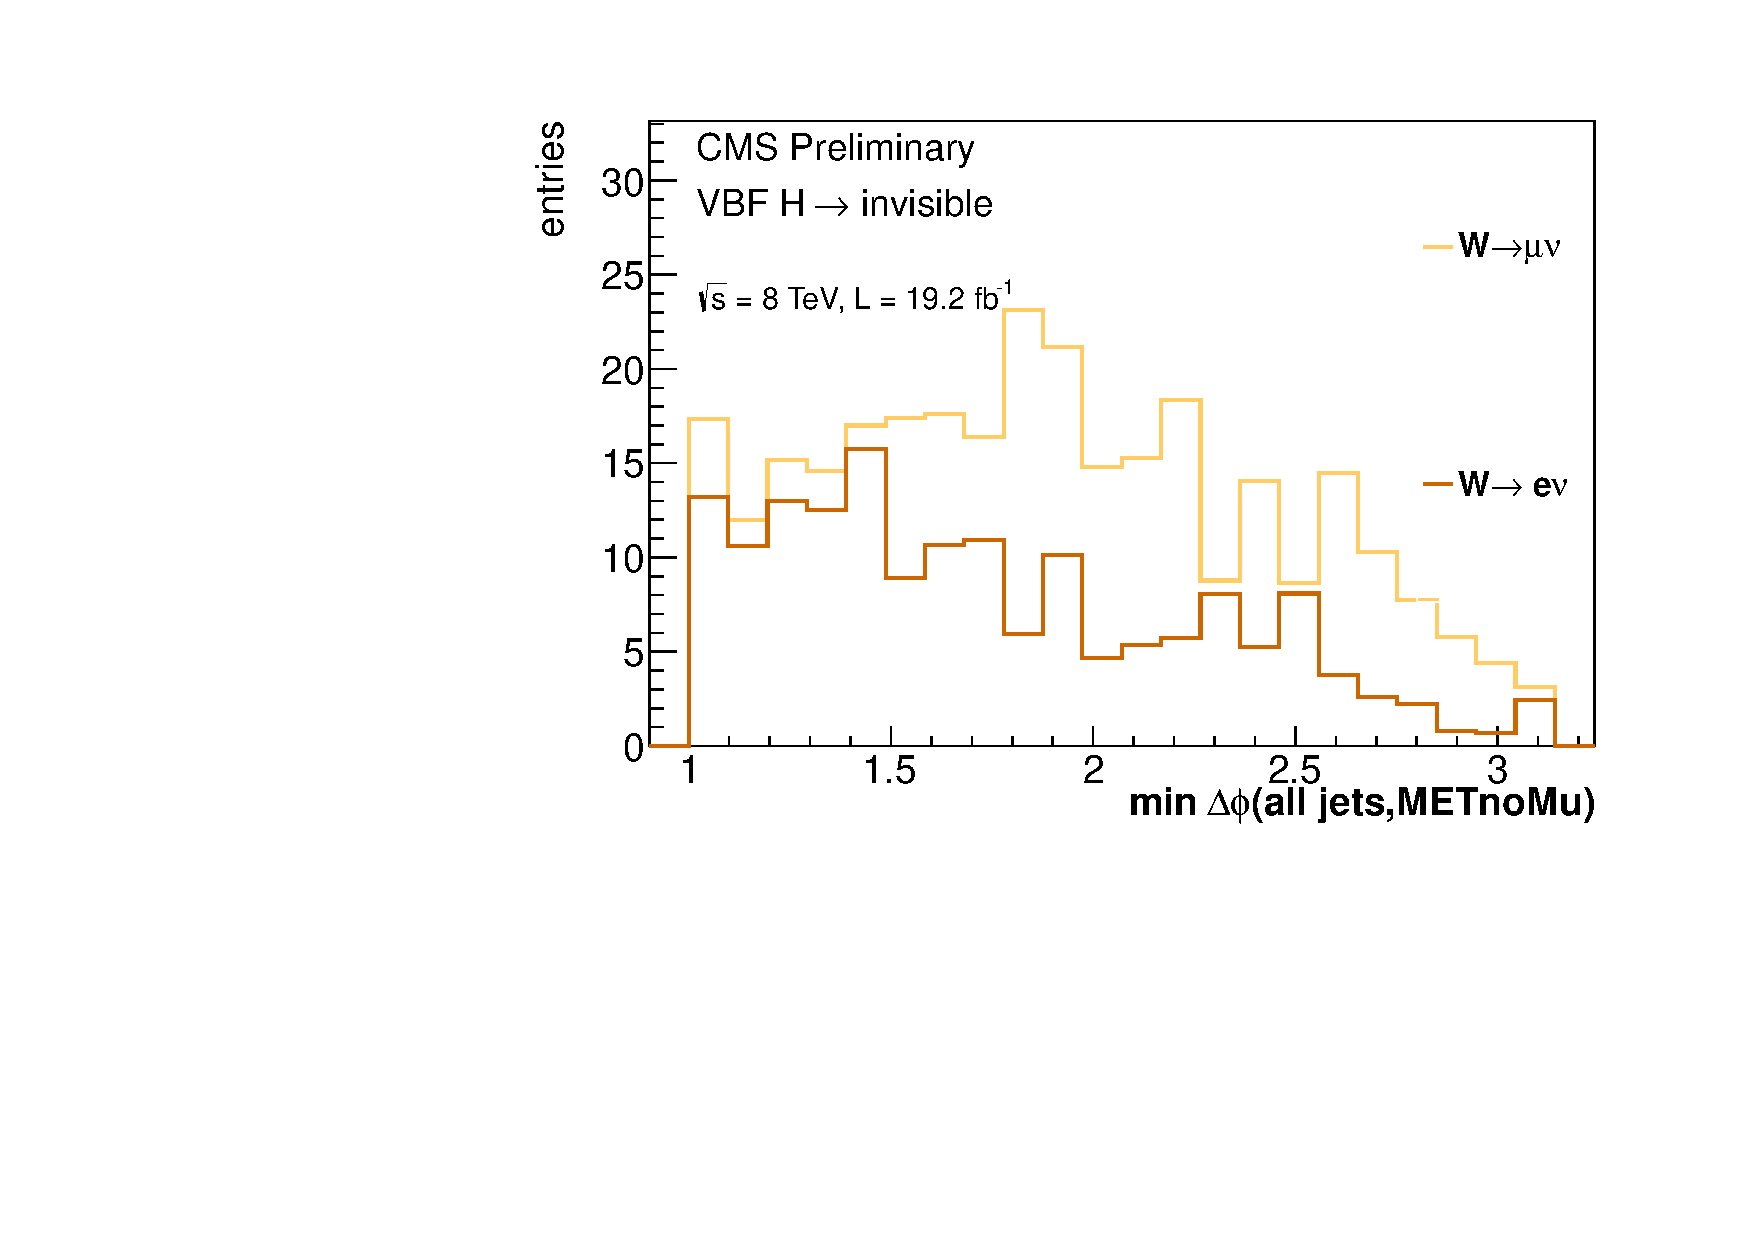
\includegraphics[width=.35\textwidth,clip=true,trim=0 0 0 30]{TalkPics/genlepstudy020315/outsideacceptance/nunu_alljetsmetnomu_mindphi.pdf}
        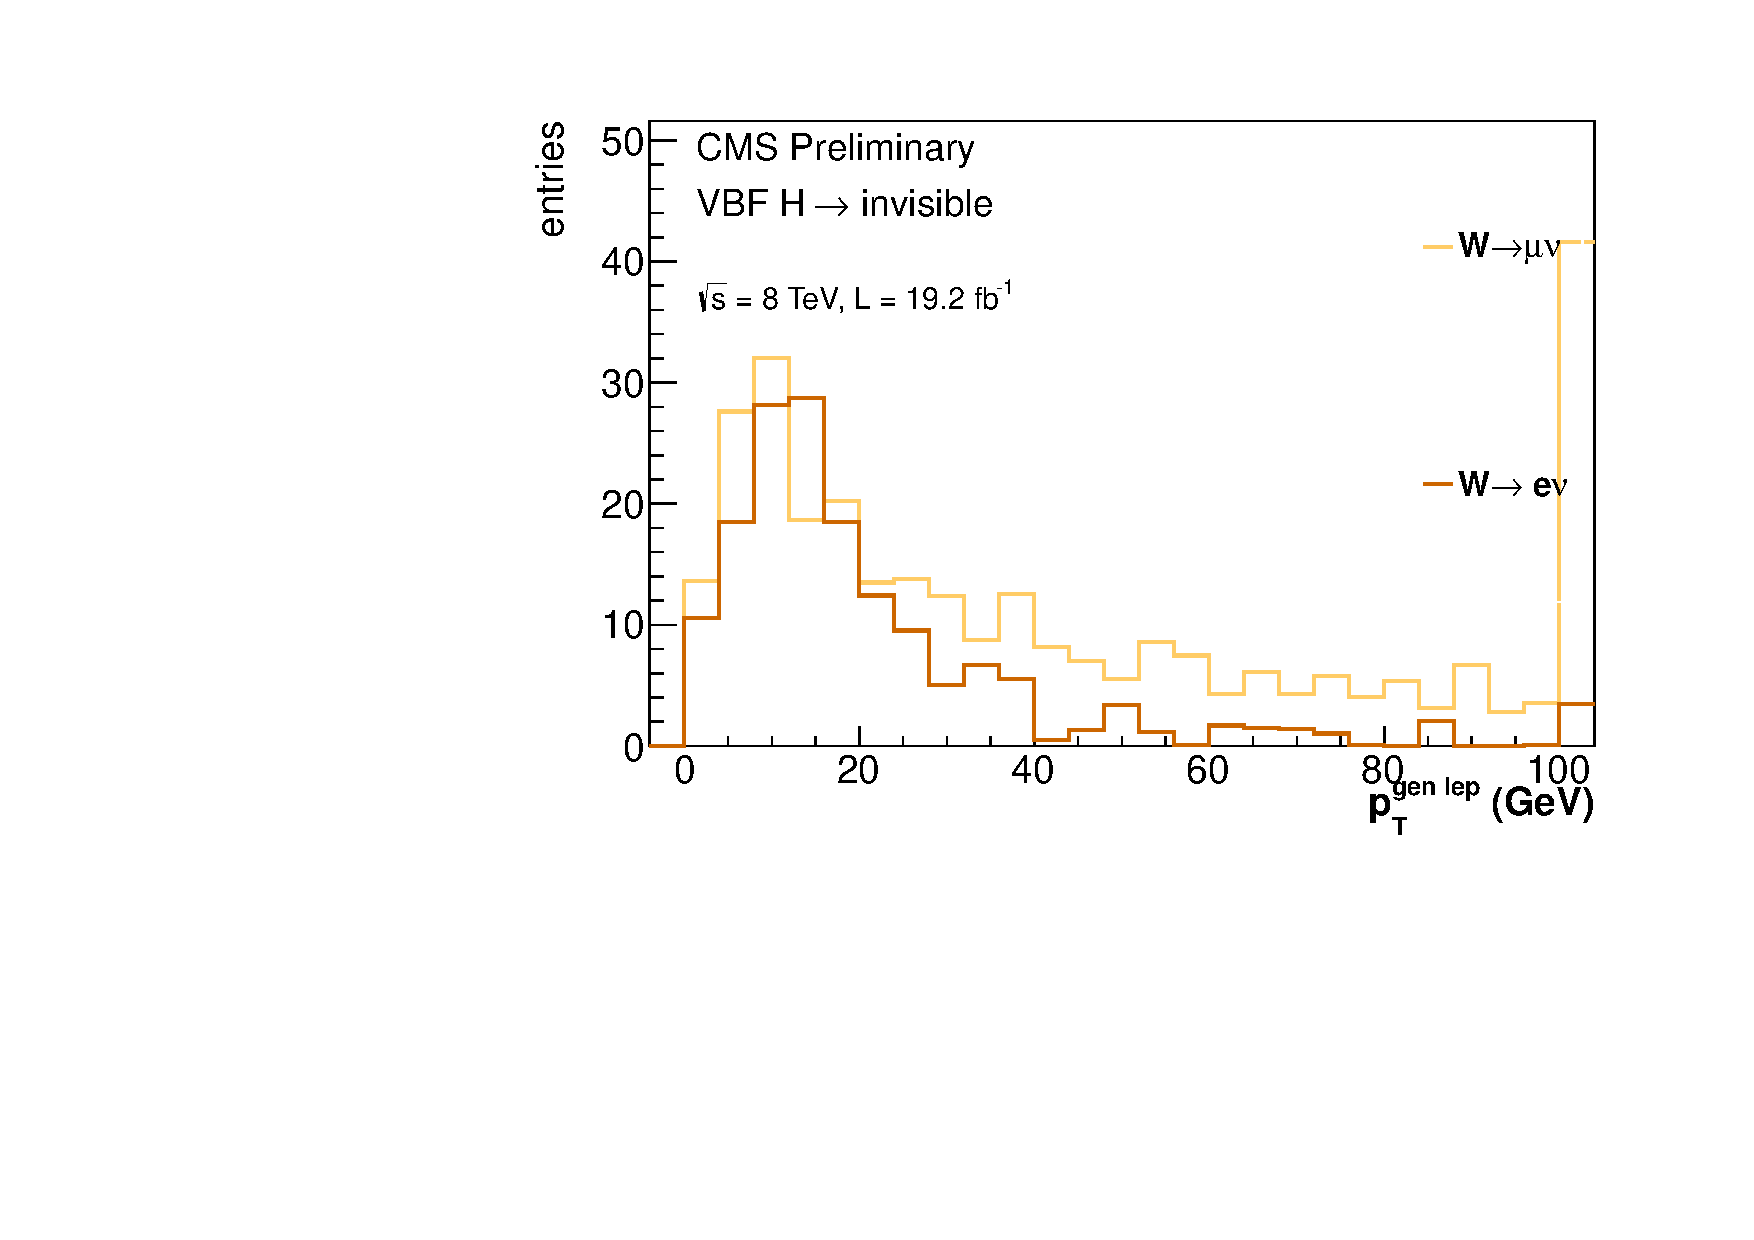
\includegraphics[width=.35\textwidth,clip=true,trim=0 0 0 30]{TalkPics/genlepstudy020315/outsideacceptance/nunu_genlep1_pt.pdf}
      \end{center}
    \end{columns}
    \begin{block}{}
      \scriptsize
      \begin{itemize}
      \item $e\nu$ events still have more jets when jetmetdphi is loosened
      \item $e\nu$ events have lower jetmetdphi than $\mu\nu$
      \item $e\nu$ Events with gen lepton $p_{T}$ much higher than 30 GeV are still failing even this looser jetmetdphi cut
      \item All consistent with hypothesis that $e\nu$ events are failing because outside acceptance electrons are often reconstructed as a jet
      \end{itemize}
    \end{block}
\end{frame}

\begin{frame}
  \frametitle{Summary}
  \label{lastframe}
  \begin{block}{}
    \scriptsize
    \begin{itemize}
    \item $W\rightarrow e\nu$ vs $W\rightarrow\mu\nu$ difference is mostly for outside acceptance events
    \item In this region unreconstructed electrons are reconstructed as jets more often than muons are
    \item These fake jets then cause events to fail our jetmetdphi cut
    \item[-] Also as the electrons deposit their energy they don't contribute to the met, so even if the event doesn't fail jetmetdphi it may not pass the met cut
    \end{itemize}
  \end{block}
\end{frame}

\begin{frame}
  \frametitle{Backup}
\end{frame}

\end{fmffile}
\end{document}
